\chapter{Evaluation}

The evaluation is conducted on several independent scenarios. As mentioned in chapter 1 the thesis relies on 4 subtask that need to be solved. First the forwarding should rely on mac addresses of the net devices and not the different faces. The second subtask is to implement a forwarding strategy that can be used with the mac addresses. The third part is to add mobility to the intermediate nodes while the fourth part is to improve on the forwarding strategy. Every scenario is evaluated and compared to ndnSIM's multicast strategy, which has been implemented in ndnSIM version 2.0 as basic multicast strategy. It basically receives an interest and forwards it to all available faces of the node except the receiving one.

To achieve comparability the scenario and trace-files are copied into a clean base installation of ndnSIM version 2.0. All parameters are kept equal. Then it is run once on the clean installation and once on the improved one. In the first scenario the implementation of the mac addresses and the forwarding mechanism is tested and evaluated. In the second scenario mobility is introduced with changes to the strategy. The different scenarios are tested for interest/data ratio, latency, congestion and number of distinct routes, although distinct routes do not exist in the already existent multicast strategy. It is introduced as part of the thesis for the new implementation.

\section{Evaluation environment}

All tests are run on the NS3 Network simulator with ndnSIM version 2.0. Different trace files are used for all the scenarios. NS2 Mobility Helper uses these trace files and adds movement to it. As Wifi standard 8011.2a was used, which means that the range is around 120 meters \cite{wifi80211a} in open space. For the propagation delay \texttt{ns3::ConstantSpeedPropagationDelayModel} was used and for the propagation loss \texttt{ns3::ThreeLogDistancePropagationLossModel} and \texttt{ns3::NakamiPropagationLossModel} were used. Interest lifetime is set to 4 seconds and the retransmission timeout to 500ms. Data packet size is 1200kb.

\section{Results for a static 8 nodes scenario}

The first scenario is a static 8 node scenario with one consumer on the left and one producer on the right. 6 intermediate nodes are placed in between as seen in figure \ref{fig:scenario1}. Every node has 3 net devices with distinct mac addresses. They allow on one hand to send and receive simultaneously while extending on the multi-path idea. The paths are determined by the mac addresses of the interest and the data. Therefore a first segement of an interest can be requested through the first net device. The second segment through the second net device and the third segment through the third net device. The fourth segement would be sent again through the first net device. That is achieved by a static counter and a modulo operation leading to different routes.

\begin{figure}[H]
  \centering
  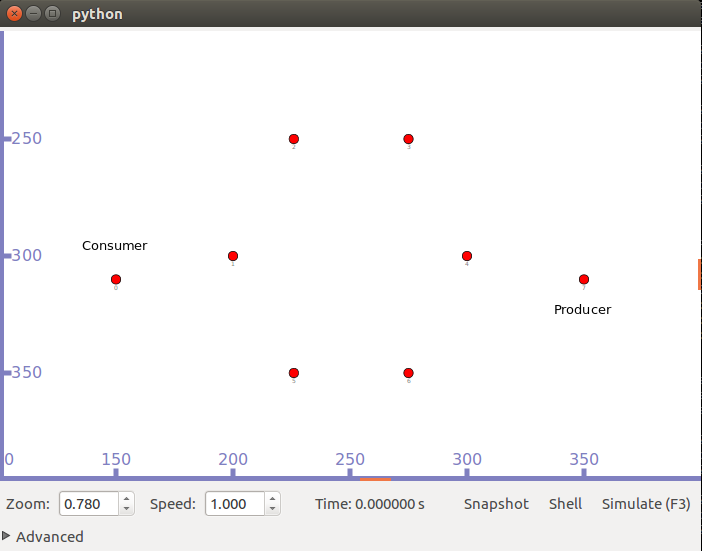
\includegraphics[scale=0.5]{chapter-5/scenario1}
  \caption{Basic static scenario with 8 nodes, 1 consumer and 1 producer}
  \label{fig:scenario1}
\end{figure}

The runs have been conducted for 100, 200, 300 and 600 seconds each. For the ratio received data over send interest only distinct packages were counted. Retransmissions were ignored. The average latency was measured in nanoseconds as the time difference of the interest leaving the consumer and the corresponding data package being received at the consumer, added together and divided by all successful interest requests.

\begin{figure}[H]
  \centering
  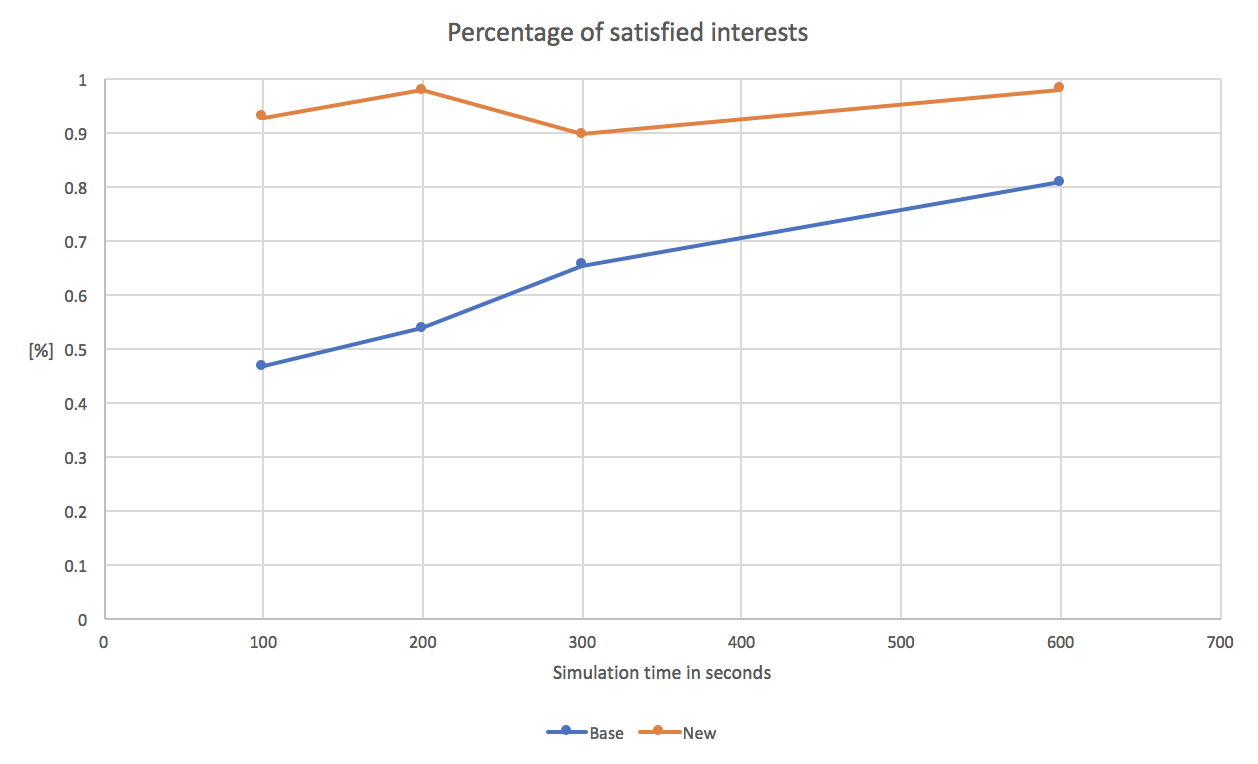
\includegraphics[scale=0.6]{chapter-5/staticS1ratio}
  \caption{Satisfaction ratio at different simulation times for both implementations}
  \label{fig:staticS1ratio}
\end{figure}

Figure \ref{fig:staticS1ratio} compares the ratio of satisfied interests (interests send / data received back) over simulation time. A better ratio has been observed for the new implementation at all simulation times. The difference is biggest at a run time of 100 seconds. At a run time of 600 seconds the difference has been reduced to 0.171. That is due to the amount of interests and data being in transition. As the number of satisfied interest constantly rises over time, the unsatisfied interest will not keep getting more since retransmissions will be made after new interests are introduced to the network.

Figure \ref{fig:staticS1iod} shows that ratio alone from figure \ref{fig:staticS1ratio} does not make any statement about the amount of the interests sent towards a potential content producer and the amount of received data. With the base implementation there is not much gain with increased simulation time whereas with the new implementation the gain nearly doubles. The reason for that observation is explained with congestion. Broadcasting the interest at each node leads to an exponential increase in the packages being retransmitted within the network leading to congestion, loss of packets and retransmissions. The new implementation floods the network only with the first interest and uses configured routes for all further interests leading to much less traffic. Retransmissions have been observed at the consumer and although the new implementation has fewer retransmissions (around 15 percent) it is not very significant and they happen on a much higher transmission rate. It can be expected that the retransmission rate is strongly correlated with the retransmission timer in the consumer and the lifetime of the interest itself.

\begin{figure}[H]
  \centering
  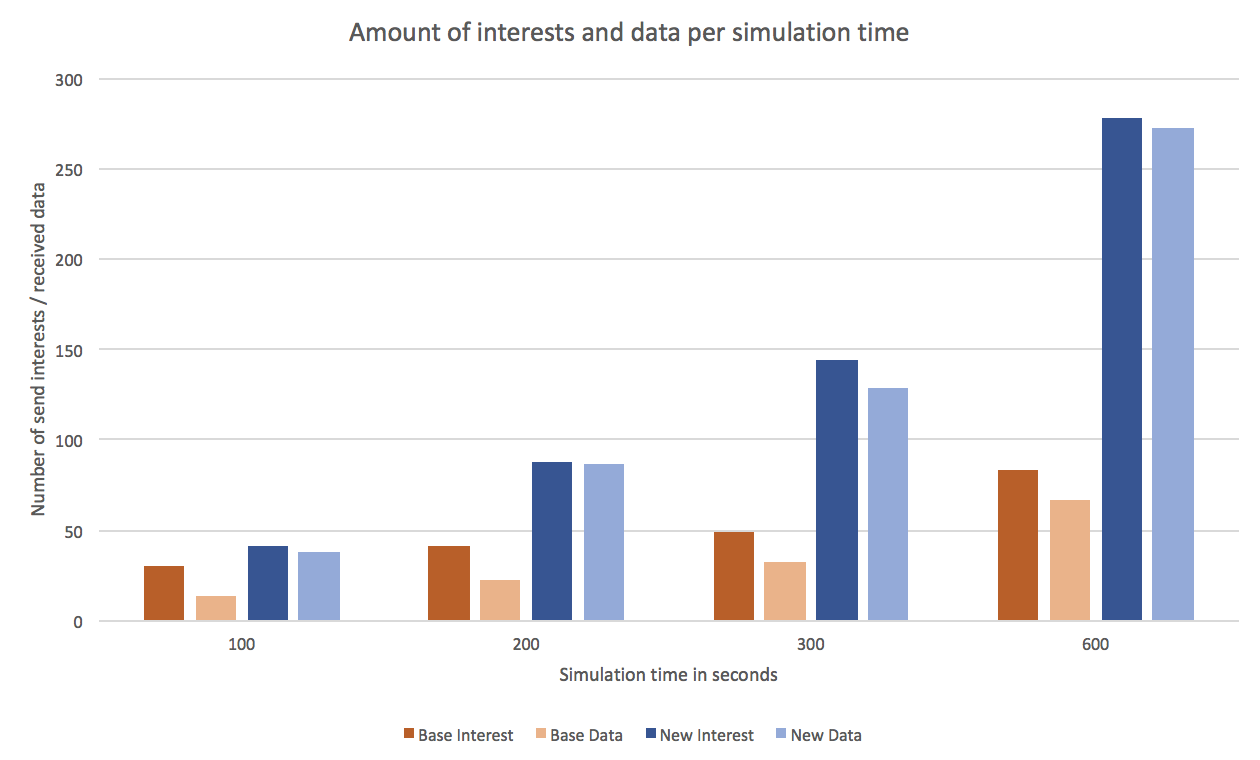
\includegraphics[scale=0.6]{chapter-5/staticS1iod}
  \caption{Number of sent and received packages over simulation time}
  \label{fig:staticS1iod}
\end{figure}

Figure \ref{fig:staticS1latency} shows how the latency changes with the simulation time and chosen implementation. As expected from \ref{fig:staticS1iod} the latency increases significantly with congestion and retransmissions in the base implementation of the multicast strategy. In the first 100 seconds it already reaches 40 seconds which multiplies by 3 at 600 seconds. The new implementation has a much lower latency starting with around 11 seconds for the first 100 seconds of the simulation. Then increases slightly till around 15 seconds for 600 seconds of simulation. That also shows that congestion and retransmission stay constant for the new implementation.

\begin{figure}[H]
  \centering
  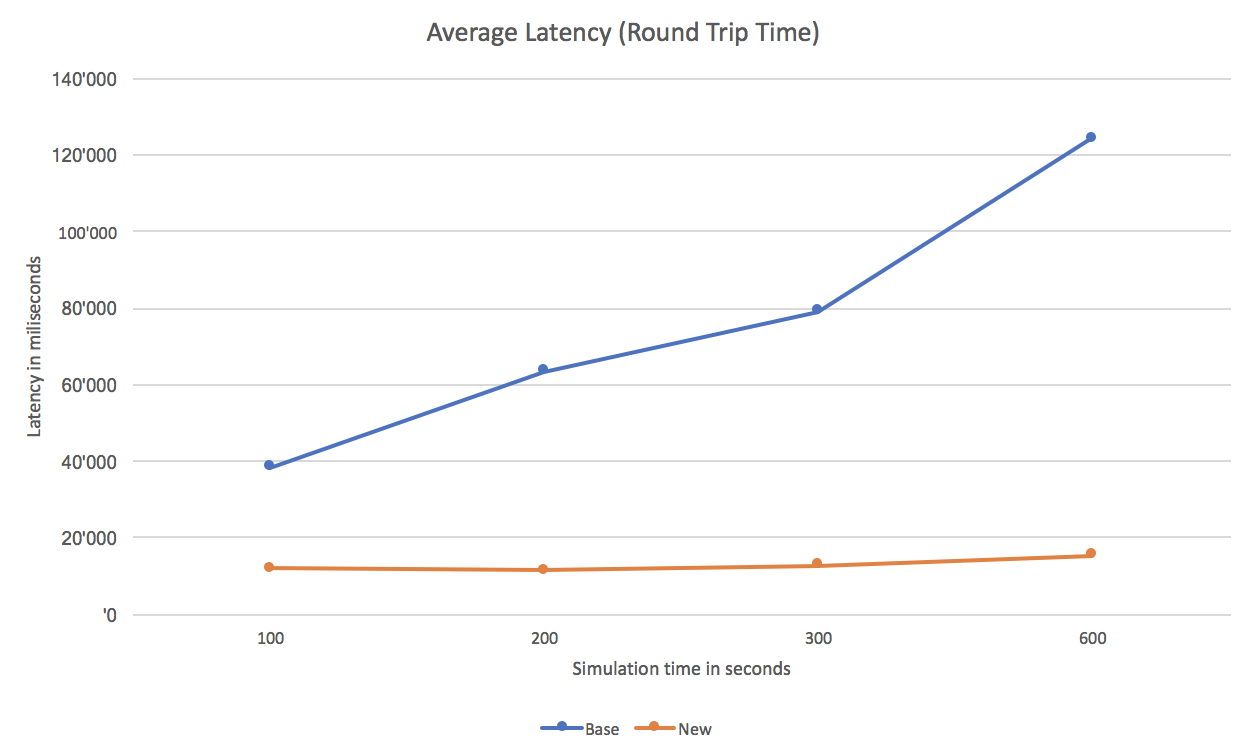
\includegraphics[scale=0.6]{chapter-5/staticS1latency}
  \caption{Latency of both implementations over simulation time}
  \label{fig:staticS1latency}
\end{figure}

The implementation has been tested with overhearing of data coming back and adding the route to the FIB entries but with a higher cost. If the data was intended for the receiving node, the node added or updated the FIB with the new information and attached cost 111 to this specific next hop. If the data was only overheard (unsolicited) a FIB entry was updated or created with cost 222 instead of ignored and dropped immediately to save resources. The results were slightly worse than the above proposed implementation but still much better than the base one.

\vspace{5mm} %5mm vertical space

Per node one to three new FIB entries were added. Another approach was to test if instead of broadcasting or forwarding the interest to only one next hop, better results would be achieved to forward the interest to two distinct next hops. This yielded again worse results and lead to the above proposed implementation.

\vspace{5mm} %5mm vertical space

One problem with more than one valid FIB entry of upstream next hops was, that after initial sorting the main routes remained the same. Instead of alternating between possible next hops only the first one was chosen and the interest forwarded to. Incrementing each cost by one after having send an interest out through that specific FIB entry made alternate the FIB entries but didn't improve the performance. It even decreased it although it led to having more distinct routes to chose from. The reason for this behaviour is how ndnSIM translates FIB entry's cost into transmission time. The lower the cost the more reliable and faster the interest is forwarded. For example setting the cost to 50 after reaching 150 while incrementing all forwarded FIB entries by one led to significantly better results then looping the cost from 250 to 150. 

\section{Results for dynamic 16 nodes scenario}

For the dynamic scenario 8 further nodes were introduced. All 14 nodes have been randomly scattered between the consumer and the producer. Random movement was added to the trace file by changing direction and speed of every intermediate node at 5 second intervals. One more net device has been added to each node to amount to a total of four net devices. 

Figure \ref{fig:scenario2} shows the topology at the beginning of the simulation. The consumer and producer are marked in the figure. Only intermediate nodes move in a random manner at different speeds. The consumer and producer have been spaced farther away from each other in order to get better and more distinct routes.

\begin{figure}[H]
  \centering
  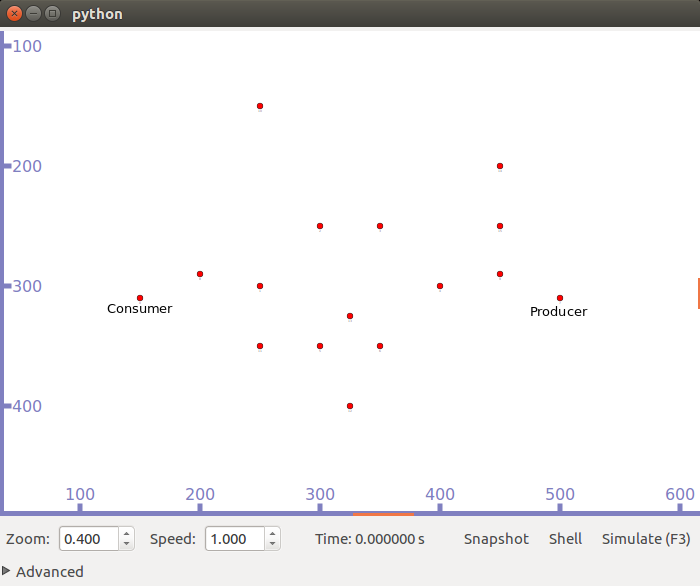
\includegraphics[scale=0.4]{chapter-5/scenario2}
  \caption{Ad-hoc scenario with 16 nodes and movement, 1 consumer and 1 producer}
  \label{fig:scenario2}
\end{figure}

Figure \ref{fig:scenario2ratio} shows ...

\begin{figure}[H]
  \centering
  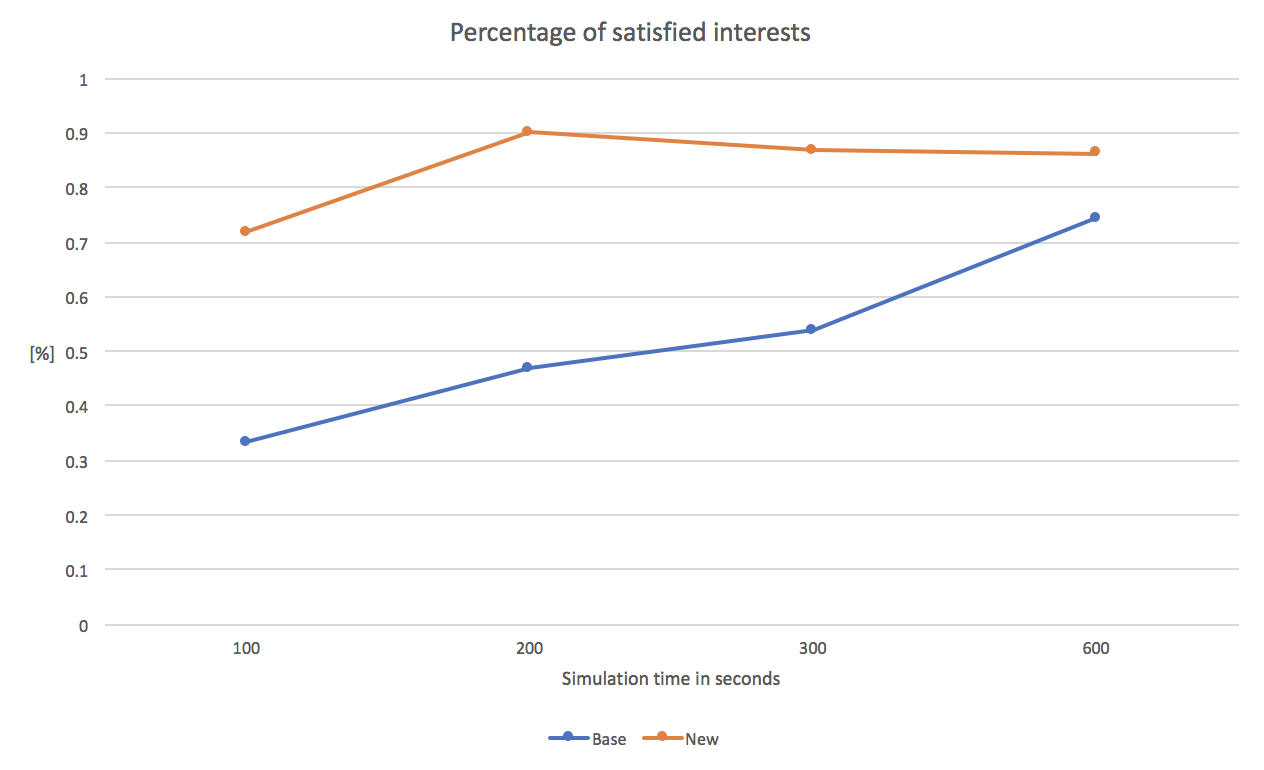
\includegraphics[scale=0.6]{chapter-5/scenario2ratio}
  \caption{Satisfaction ratio at different simulation times for both implementations with mobility}
  \label{fig:scenario2ratio}
\end{figure}

Figure \ref{fig:scenario2iod} shows....

\begin{figure}[H]
  \centering
  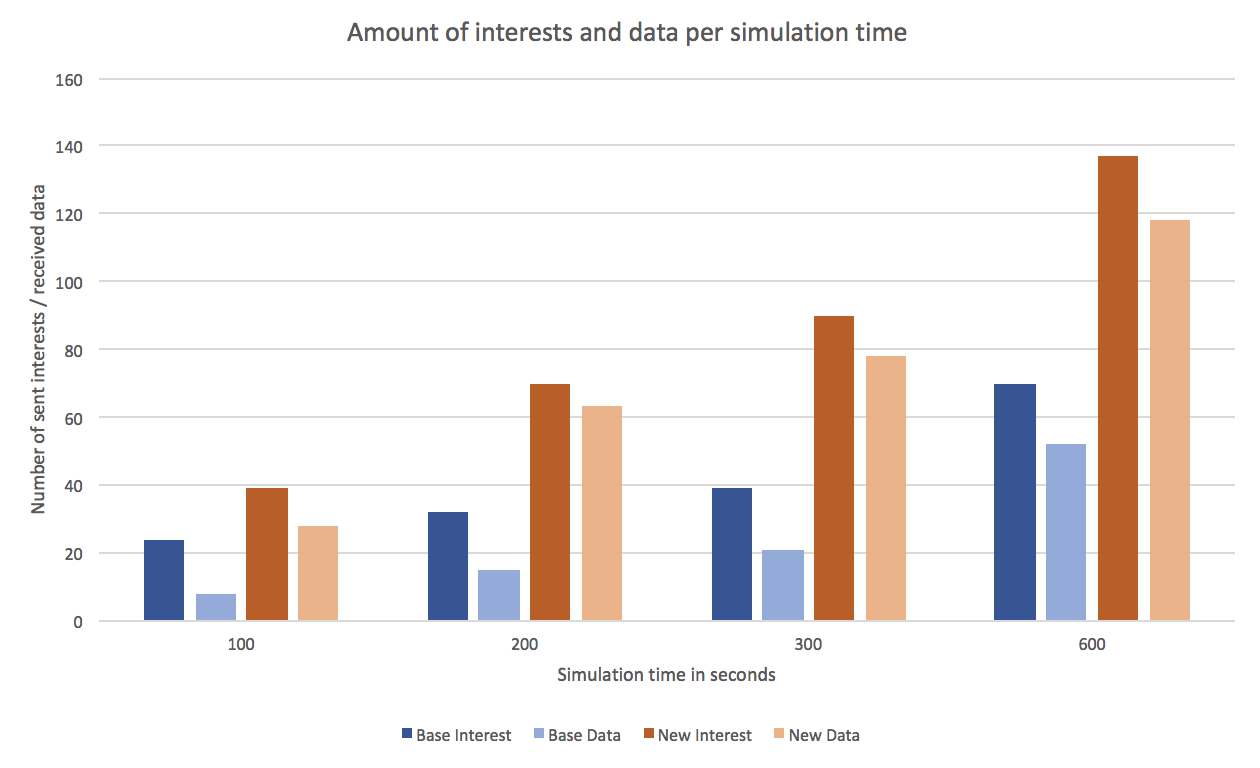
\includegraphics[scale=0.6]{chapter-5/scenario2iod}
  \caption{Number of sent and received packages over simulation time}
  \label{fig:scenario2iod}
\end{figure}

Figure \ref{fig:scenario2latency} shows....

\begin{figure}[H]
  \centering
  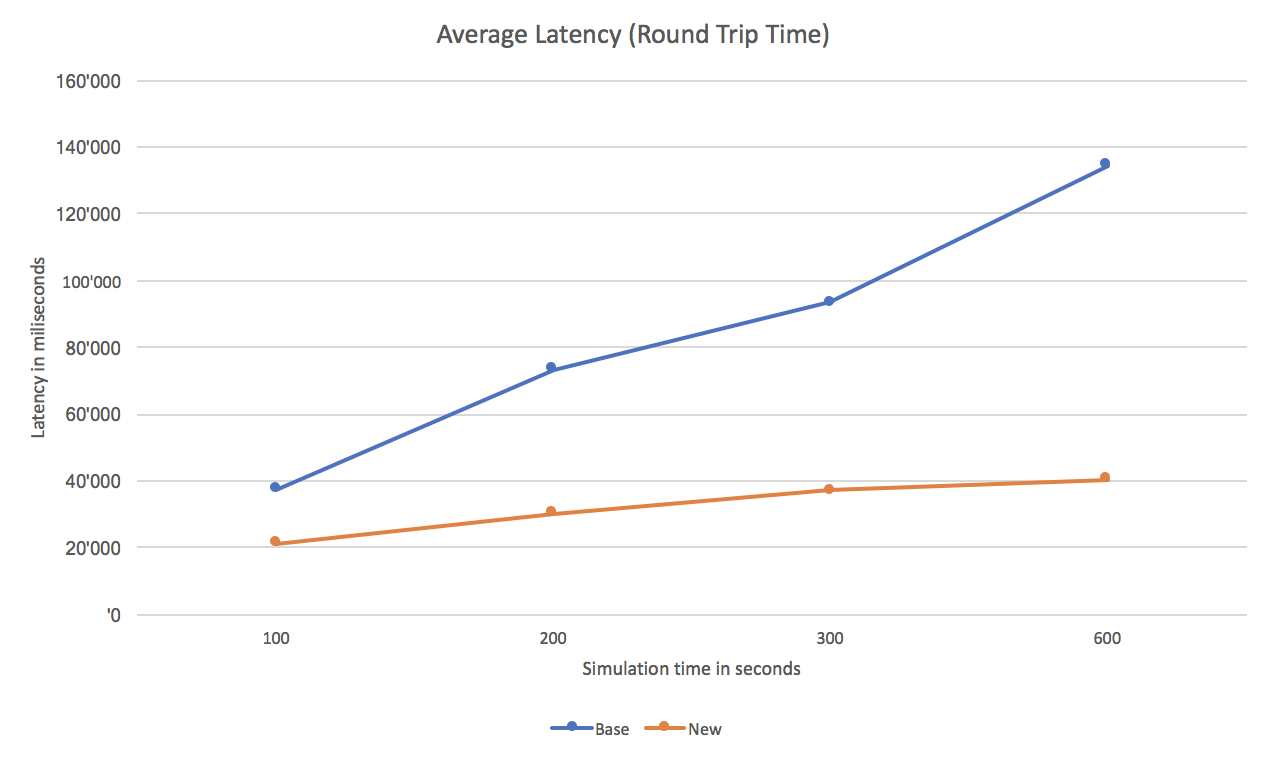
\includegraphics[scale=0.6]{chapter-5/scenario2latency}
  \caption{Latency of both implementations over simulation time}
  \label{fig:scenario2latency}
\end{figure}






